\documentclass[12pt,onecolumn,letterpaper,draftclsnofoot]{article}

\usepackage{cvpr}
\usepackage{times}
\usepackage{epsfig}
\usepackage{graphicx}
\usepackage{amsmath}
\usepackage{amssymb}
\usepackage{booktabs}
\usepackage{multirow}
\usepackage{subcaption}
\usepackage{scrextend}
\usepackage{bm}

% Include other packages here, before hyperref.

% If you comment hyperref and then uncomment it, you should delete
% egpaper.aux before re-running latex.  (Or just hit 'q' on the first latex
% run, let it finish, and you should be clear).
\usepackage[breaklinks=true,bookmarks=false]{hyperref}

\DeclareGraphicsExtensions{.pdf,.jpg,.png,.jpeg}
\graphicspath{{images/}, {figs/}}
\newcommand{\todo}[1]{\textcolor{red}{{\em [#1]}} }
\newcommand{\specialcell}[2][c]{%
    \begin{tabular}[#1]{@{}c@{}}#2\end{tabular}}
\newcommand{\secref}[1]{Section~\ref{sec:#1}}
\newcommand{\figref}[1]{Figure~\ref{fig:#1}}
\newcommand{\tabref}[1]{Table~\ref{tab:#1}}
\newcommand{\equref}[1]{Equation~\ref{equ:#1}}
\newcommand{\matr}[1]{\mathbf{#1}}
\newcommand{\bfit}[1]{\boldsymbol{#1}}
\newcommand{\bs}[1]{\boldsymbol{#1}}

\DeclareMathOperator*{\argmax}{arg\,max}
\DeclareMathOperator*{\argmin}{arg\,min}

\cvprfinalcopy % *** Uncomment this line for the final submission

\def\cvprPaperID{****} % *** Enter the CVPR Paper ID here
\def\httilde{\mbox{\tt\raisebox{-.5ex}{\symbol{126}}}}

% Pages are numbered in submission mode, and unnumbered in camera-ready
%\ifcvprfinal\pagestyle{empty}\fi
%\setcounter{page}{4321}
\begin{document}

%%%%%%%%% TITLE
\title{Sound Absorption of Rooms}

\author{Weilian Song\\
University of Kentucky\\
% {\tt\small firstauthor@i1.org}
% For a paper whose authors are all at the same institution,
% omit the following lines up until the closing ``}''.
% Additional authors and addresses can be added with ``\and'',
% just like the second author.
% To save space, use either the email address or home page, not both
}

\maketitle
%\thispagestyle{empty}

%%%%%%%%% BODY TEXT
\section{Introduction}

A lot of the music we hear today are exceptionally clear, with very little
noise that is only audible with very good equipment. However, whenever we as
students do a project involving audio recording, it always sounds like there's
static noise in the background. While there can be many reasons why our
recorded audio is noisy, the main issue is that the environment in which we
record at does not absorb sound very well, and can cause unwanted noise to
reflect back to the recording device or make wanted noise diminish into
nonexistance. Understanding how different rooms absorbs sound will prove
useful in the future whenever audio recording is necessary, to provide the
clearest possible sound for the intended application.

There are three obvious factors when determining room sound absorption level:
size, number of objects in the room, and materials of the objects and walls.
Size determines how fast sound waves bounce back to the recording device;
number of objects in the room determines how often the sound wave has to
bounce before reaching the recording device, and materials of various objects
and walls determine the amount of sound that gets reflected.

With the three factors as our independent variables and the sound absorption
level as our dependent variable, I hypothesize that the sound absorption level
is higher with:

\begin{enumerate}
  \item Bigger room
  \item More objects in the room
  \item Materials with rougher or special designed surfaces
\end{enumerate}

In this paper, we explore the sound absorption characteristics of four 
different rooms: a compact dormatory room, a large classroom, a large concert
hall, and an anechoic room designed specifically for sound recording. For each
room we will be playing three sounds at different frequencies to also determine
the correlation between frequency and absorption level.

\section{Related Work}

\paragraph{Absorption Properties of Materials}
Extensive research has been conducted to determine the sound absorption
properties of various materials. \todo{cite} Asdrubali et.\ al.\ \todo{cite
here} experimented with the absorption properties of recycled rubber crumbs
from old tyres. Their independent variables include the grain size, compaction
ratio, thickness of the end product, and bonding agent used to adhere the
rubber grains together. In their research they discovered that small sized
rubber grains, purposely developed resin, 20\% compaction ratio and thickness
of 9.4 cm works the best for sound absorption.
%
\begin{figure}
  \centering
  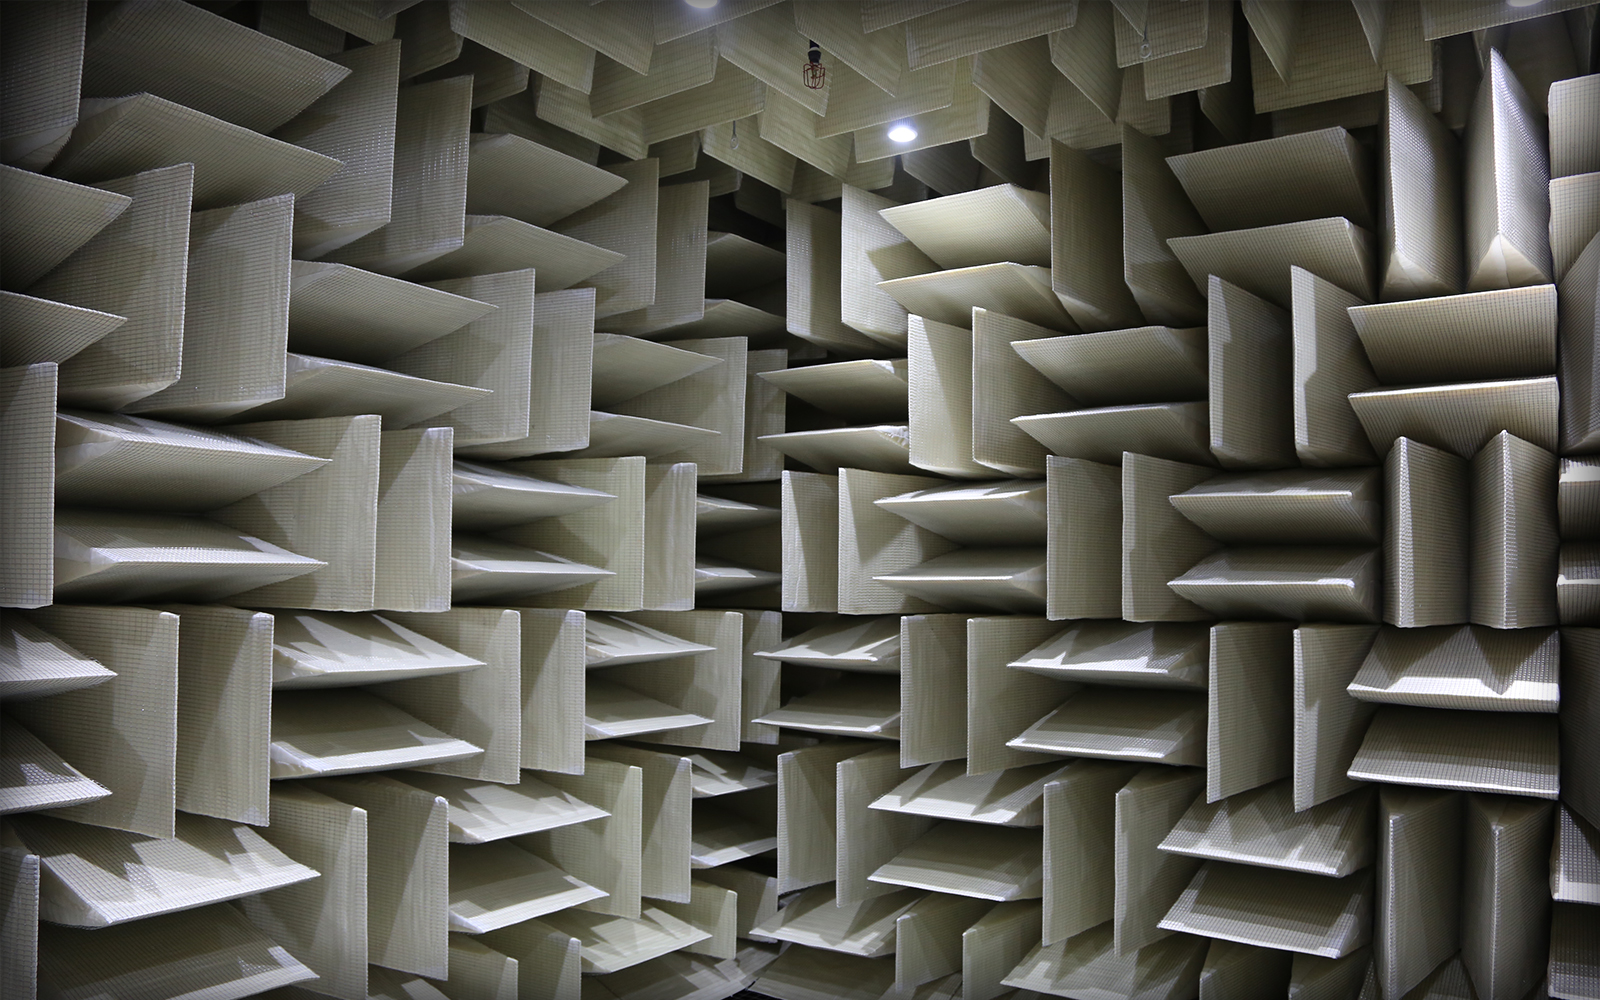
\includegraphics[width=0.5\linewidth]{chamber}
  \caption{Inside of an anechoic chamber, borrowed from \todo{cite}}
  \label{fig:chamber}
\end{figure}

\paragraph{Room Absorption} 
Room sound absorption can be expressed in terms of the room's sound absorption
coefficient. As explained in \todo{cite}, given that we know the room walls'
materials, we can perform a lookup of each material's sound absorption
coefficient $\alpha$ through the provided table in \todo{cite}, and calculate
the total room sound absorption $A$ with the following equation:
%
\begin{equation}
  A = \sum_{i} S_i \alpha_i
\end{equation}
%
where $S_i$ is the total area of material $i$ in unit $m^2$ and $\alpha_i$ is
the sound absorption coefficient for material $i$. Mean absorption coefficient
for every $m^2$ of the room can be calculated through dividing $A$ by the
total area of the room.

Sound absorption coefficient is a good way to measure a room's acoustic
niceness, as it provides a quantifiable metric for comparing rooms with
different sizes and materials.

Different materials within the room will absorb different amounts of sound.
For example Asdrubali et. al. experimented with the absorption properties of
recycled rubber crumbs from old tyres. Their independent variables include the
grain size, compaction ratio, thickness of the end product, and bonding agent
used to adhere the rubber grains together. 

\paragraph{Anechoic Chamber}
For recording and research purposes, there are rooms specifically designed for
maximum sound absorption, which are called anechoic chambers, as shown in
\figref{chamber}. \todo{cite} Construction of a world-class anechoic chamber
is extremely tedious, having to consider many aspects like location of the
chamber, size of the room, materials of the wall, custom parts, etc. The
eStudio on campus also has a small anechoic chamber, elevated off the ground
for less transmitted vibration and lined with foam sound absorption materials
on the inside to remove echo.

\section{Methods}
The goal of the experiment is to identify the effect of room sizes and
materials on sound absorption. To achieve that goal, three rooms with
different sizes and materials are chosen: small, medium and large. The small
room is my dorm room, which is compact, non-echoic and has smooth walls with
dense object arrangements. The medium room is a medium classroom, which is
slightly echoic and is relatively open. Finally the large room is a large
classroom, with rough brick walls, echoic room characteristics and is very
open.

To measure the sound absorption level of the room, a microphone and a speaker
is placed in the center of the room, with the speaker and the microphone
placed ??? inches apart. A simple overview of the setup is shown in
\figref{setup} \todo{figure out how far they are} 
%
\begin{figure}
  \centering
  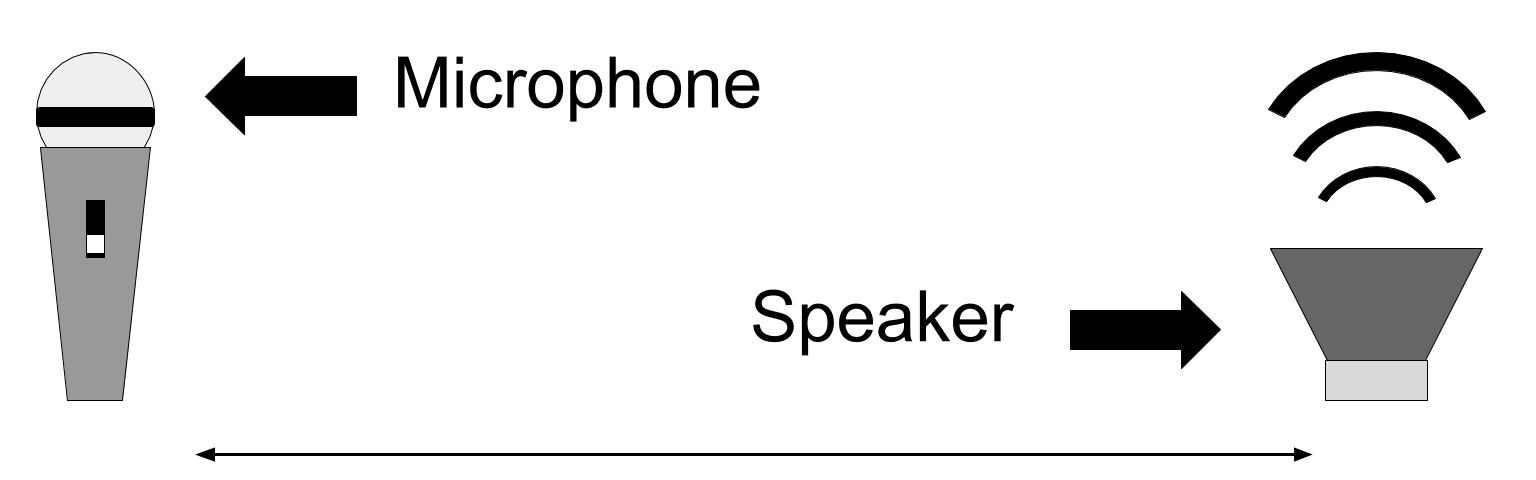
\includegraphics[width=0.5\linewidth]{setup}
  \caption{Experiment setup}
  \label{fig:setup}
\end{figure}
%
Four measurements are taken for each room, one with the speaker turned off
(ambient noise), and three with the speaker playing sound at 500, 2000 and
4000 Hz. The purpose of the different sound frequencies is to discover if they
are different in terms of percentage of absorption. Each measurement is ten 
seconds long, and with three different rooms, a total if twelve audio clips
are recorded.

\section{Experiment}

For the recording device, a Blue Yeti microphone is used, with gain set at
100\% and pickup pattern set in omnidirectional mode. For the speaker, an
iPhone is used, playing the three frequencies at max volume. To record the
audio, the microphone is plugged into a laptop and a simple python scrip is
used to save and analyze the recorded audio clips.

\section{Conclusion}

{\small
\bibliographystyle{ieee}
\bibliography{biblio}
}

\end{document}
